% \documentclass[12pt]{template}

\begin{document}   
\section{事件描述对事件参与人数的影响} 
\subsection{概述}  
在\textit{EBSN}中,对于一个组织者,一个非常重要的问题就是如何使自己的活动更受欢迎,借而吸引更多的人参加。而决定一件事件的属性则是相当繁复的,例如事件主题,举办时间,地点,所在组,事件描述等。作为这些属性中自由度最大的属性之一,问题描述在提高事件吸引力上所起的作用是相当显著的。例如下面
两段事件描述,从直觉上来说,第一段描述显然比第二段更有活力。而事实也是如此,第一
个事件的参与人数(超过97\%的同类事件)要远高于后者(超过5\%的同类事件)。因此,如何写出出色的事件描述,对于事件举办者而言,是个相当重要的技巧。
 
\begin{quotation}
  \textit{let  \'s get ready to get in our bikinis and board shorts  (  spe
  edos for the europeans  )  and enjoy the la summer heat on the beach
  !  this year the event is on saturday  ,  august 10th starting at 
  1pm . we will have muchies  ,  drinks and games . for those that 
  are into volleyball  ,  let  \'s repeat what we did last year . 
  i saw a lot of losers  ,  i mean winners. lol . let  \'s enjoy 
  a few good volleyball game . \\ 
  }
    
  \textit{open to the public for a group class package and individual classes}
\end{quotation}

但是想要去定量研究事件描述对事件参与度的影响,又是相当困难的。一方面是因为事件描述是自然语言,难以建模,虽然近年出现了诸如词向量(\textit{word embedding}),时序网络(\textit{RNN})等手段,较好的克服了传统的自然语言处理中的一些问题(例如反义词),并在机器翻译,文本生成等领域取得了不错的效果,但这些方法并不能很好的解决语义一致性的问题,例如在文本空间中,\textit{(this flower smells pretty)} 和 \textit{this flower smells pretty bad}会比较接近,但它们的意思是截然不同的。另外,这些方法的本质还是去拟合文本序列的概率分布,以最大化某个目标函数的期望或概率,因此很难说它们是真正理解了语义。这两方面使想要定量研究事件描述的作用变得格外困难。

在这一章中,为了解决以上问题,我们提出了事件相似度的定义,并使用了简单但可解释的拉索回归对文本进行分析。提出事件相似度是因为事件的复杂性使我们必须采用合适的手段来对事件进行分类并分别度量。例如无论事件描述的好坏,一场讲座的参与人数总会比一次小型聚会来的多。所以简单的使用同一度量手段将以上两种事件一起衡量是不准确也不公平的。而这里不使用更为复杂的模型例如时序网络的原因则是受\cite{noauthor_predicting_nodate}启发,我们想观察是描述中的哪些成分对参与度有影响。比如同为聚会,包含drink的聚会是否会比包含church的聚会有更多的参与人数。而这方面的信息是可以从拉索回归中的系数获得的。

本章接下来的结构如下:在第二节,我们会定义问题并建立模型,其中会对\textit{meetup}中的属性做详细的解释,第三节会对描述文本建模,并使用拉索回归来寻找对事件成功起关键性的词,第四节则介绍了事件相似度及事件相似矩阵的定义,第五节则用来证明文本质量会对事件成功产生影响。

\subsection{问题描述}
\subsubsection{数据集}

meetup\footnote{http://www.meetup.com/about},和豆瓣小组类似,是一家提供在线组织活动的平台。\textit{meetup}中有三个基本对象:用户,小组,事件。具有相同兴趣的用户聚在一起组成小组,而用户也可以在小组中发布事件。用户通过RSVP来回复是否参与该事件。有些小组内的事件仅开放给组员参加,有些则对公众开放。我们使用了meetup上的api爬取了meetup在LA的部分数据,包括当地的组,组内成员信息及组的历史事件。具体信息如表(\ref{t1})。
\begin{table}[htbp]
  \label{t1}
  \caption{LA中近两年的meetup数据}
  \begin{center}
    \begin{tabular*}{\linewidth}{p{0.5\linewidth}p{0.5\linewidth}}
\toprule
    & LA\\
\midrule
    Users & 172673\\
    Events & 166829\\
    Groups & 2507\\
\bottomrule
    \end{tabular*}
  \end{center}
\end{table}

我们使用一个七元组来表示\textit{meetup}中的一个事件\(e_{id}(id,t,d,h,a,l,c)\),其中\(t\)是事件举办时间,\(d\)是事件描述,\(h\)是事件所在组,\(a\)是事件参与人,\(l\)是事件所在地点。\(c\)是事件主题:meetup的事件有36个主题。以及三元组来表示组\(g_{id}(id,e,m,c)\),其中\(e\)是事件,\(m\)是组内成员,\(c\)是该组的主题。注意到这里并没有关注成员和组的兴趣标签,虽然它在事件安排和事件推荐中的作用非常大,但在本文显然不是值得注意的信息。

在解释了上述对象和属性后,我们就可以给该问题完整的下一个问题定义了。

\subsection{问题定义}
\textbf{定义一: 成功事件}指对于一个事件\(e_{id}\)和与其相似的事件\(E\{e_1,e_2,e_3,...\}\),
\(|e_{id}^a|\)大于\(E\)中\(70\)\%的事件。

衡量事件成功的因素有很多,这里之所以采用参与人数是因为我们想要研究的是事件参与度,而参与人数相较于其他属性则是比较直观且准确的数值,借助于此我们可以准确的衡量一个事件在事件参与度上的表现。而且对于绝大多数事件举办者来说,如果事件参与人数超过了同类事件的百分之七十五,那么该事件可以算得上是成功事件了。

\textbf{定义二: 相同事件}指对于事件\(e_{id_1}\)和事件\(e_{id_2}\),\(e_{id_1}^d=e_{id_2}^d\)

在meetup中有大约30\%的事件属于相同事件,它们对于推荐算法意义重大,但如果只为了考察事件描述对事件成功的影响,则会起到相反的作用。因为在衡量事件描述产生的影响时,该类事件会增加其事件描述的影响比重,进而导致结果偏向于重复出现的事件描述。其二是参与这类事件的人有着很大的重叠,他们是基于经历而不是基于事件描述来选择参与该事件的,所以他们对事件描述不敏感。因此剔除该类事件是有必要的。对于相同事件,我们只保留其平均值。

\textbf{定义三: 相似事件}
指对于事件\(e_{id_1}\)和事件\(e_{id_2}\),\(sim(e_{id_1},e_{id_2})>\gamma\),其中\(sim\)是相似矩阵,\(\gamma\)是阈值。关于相似矩阵建立和阈值的选择可以在第\ref{4}节看到。

根据以上的三个定义,最终的问题定义如下:

\textbf{定义四: 问题定义}

给定事件\(e_{id}\)和相似事件\(E\{e_1,e_2,...\}\),判断\(|e_{id}^a|\)
是否超过了\(E\)中70\%的事件。由此可见,我们把该问题转化成了一个预测问题。

\subsection{文本建模}

\subsubsection{独热编码}

独热编码是文本编码方式中最简单的一种,通过给每一个词一个独特的id并在词向量中的对应位置一,我们便获得了每一个词的独有编码。独热编码有着诸多缺点,例如词向量间是正交的,因此此编码方式无法表现词与词的关联。但是其优点也十分明显:简单。此处采用该编码方式的原因正因如此。

\subsubsection{拉索回归}

拉索回归是线性回归的一种,与传统线性回归的损失函数不同的是,它的损失函数中包含了其回归系数的绝对值的罚函数。由于其采用了罚函数的绝对值而非平方,导致其一些系数归零,可以借此选出些重要的变量\cite{tibshirani_regression_1996},因此我们可以对参与人数进行回归,来挑选出对参与人数影响比较大的单词\cite{noauthor_predicting_nodate}。
\begin{equation}
argmin\left\{\displaystyle\sum_{i=1}^N\left(y_i-\beta_0-\displaystyle\sum_j\beta_jx_{ij}\right)\right\}
\end{equation}
\begin{equation}
subject\ to \displaystyle\sum_j|\beta_j|\leq\alpha\
\end{equation}

其中\(y_i\)为第\(i\)个目标即参与人数,\(x_{ij}\)为\(e_i^d\)中第\(j\)个单词。\(\alpha,\beta_0\)为预先设定的参数。
\subsection{文本处理}\label{3.2}

这里我们使用独热编码对文本建模,并去除停止词和非英文单词。我们希望使用拉索回归来寻找对参与人数影响最大的
单词,并得到一个可以解释的结果。因此我们需要确定合适的惩罚系数,使大多数参数归零。为了找到合适的参数,我们使用了网格搜索和交叉验证的方式,最终发现惩罚系数在1.236*1e-1的时候结果最为理想。在这次实验中,我们随机挑选了100个组,其中包含了8673个事件,去除相同事件后还剩5579个事件。将这些事件的事件描述作为输入,对它们的参与人数进行回归后挑选出了系数最高和最低的8个词,如表(\ref{t2})所示,需要注意的是这里并没有考虑其他事件属性对参与人数的影响。

\begin{table}[htbp]
\label{t2}
\caption{对参与人数的影响比较重要的词}

  \begin{center}
    \begin{tabular*}{\linewidth}{p{0.15\linewidth}p{0.35\linewidth}p{0.35\linewidth}p{0.15\linewidth}}
\toprule      
    &系数最高的8个词 & 系数最低的8个词&\tabularnewline
\midrule
&christmas & week&\tabularnewline
&dance & saga&\tabularnewline
&directions & meditation&\tabularnewline
&cocktails & information&\tabularnewline
&concerts & salt&\tabularnewline
&band & mammoth&\tabularnewline
&perfect & spiritual&\tabularnewline
&tribute & masked&\tabularnewline
&drinks & learn&\tabularnewline
\bottomrule
    \end{tabular*}
  \end{center}
\end{table}
  
其中有些词符合人的主观判断,例如cocktails,drinks等,有些则不那么直观,比如spiritual(这个词出现在一个教堂组织的礼拜活动中),不过这个实验结果从某些程度上印证了我们的猜想:在聚会活动中,一起开party显然比一起做礼拜要有吸引力。

然而简单的对所有事件做回归是一种不公平的做法,因为有些种类的活动,例如喝下午茶,其参与人数和另一些活动例如踢足球,有着先天的区别。因此有必要将不同的事件分开来,让比较仅在相似的事件间进行。因此,如何找到相似的事件便变得重要了。在接下来的一节,我们将给出一系列相似矩阵的定义,从而最终得到事件的相似矩阵。

\subsection{事件相似度}
由meetup上爬取的数据来看,一个事件由时间,地点,主题,举办者,举办组等属性决定,因此,我们可以通过定义这些属性的相似度来反推事件的相似度。

\subsubsection{举办组的相似度}
两个组的相似可以分为两个方面,一是组的主题相似,二是组的成员相似。分别的,我们对应定义了两个矩阵:

\textbf{(1) 主题相似度} \(group\_cat\_sim:\)

\begin{equation}
group\_cat\_sim(i,j)=\frac{|g_i^c\bigcap g_j^c|}{|g_i^c|}
\end{equation}


\textbf{(2) 成员相似度} \(group\_mem\_sim:\)

\begin{equation}
group\_mem\_sim(i,j)=\frac{|g_i^m\bigcap g_j^m|}{|g_i^m|}
\end{equation}

通过这两个矩阵的线性组合,我们就能衡量出两个组间的相似度。

\subsubsection{事件主题相似度}

和组主题相似度类似,定义如下:

\begin{equation}
event\_cat\_sim(i,j)=\frac{|e_i^c\bigcap e_j^c|}{|e_i^c|}
\end{equation}

\subsubsection{时间相似度}

我们希望相似的事件在时间上也更接近,时间相似度越大。同时我们也希望确保时间相似度的值域能在\([0,1)\)之间,因此,使用负指数函数。

\begin{equation}   
time\_sim(i,j)=\mathrm{e}^\frac{-|e_i^t-e_j^t|}{\alpha}
\end{equation}

其中\(\alpha\)为参数。

\subsubsection{地点相似度}

同样的,距离越近的事件地点相似度越高。这里使用haversine公式计算出两点之间的距离

\begin{equation}   
loc\_sim(i,j)=\mathrm{e}^\frac{-|e_i^l-e_j^l|}{\alpha}
\end{equation}

\subsubsection{事件相似度}
基于以上5个矩阵,我们定义如下事件相似矩阵:

\begin{equation}   
  \begin{split}
event\_sim(i,j)=\alpha*group\_mem\_sim+\beta*group\_cat\_sim
+{c}*time\_sim+{d}*loc\_sim+{e}*event\_cat\_sim
  \end{split}
\end{equation}

其中\(\{\alpha,\beta,{c},{d},{e}\}\)都是归一化后的参数,至于阈值\(\gamma\)的选择则应该参考\(event\_sim\)的值的分布,在实验中我们使用了前20\%的数值。

我们在定义相似矩阵的时候,主要依据的是人的主观想法:两件事件,如果主题相似,距离相近,时间相近,所在组相似(相同),那么它们很有可能是相似的。相应的,我们希望一件能借助相似矩阵来排除掉百分之80以上的其他事件,而实验结果也正是如此。

\subsection{实验}

\subsubsection{实验设计}
为了考察事件描述对事件成功的影响,我们设计了如下实验:首先,使用第\ref{4}节定义的\(event\_sim\)选出相似的事件。然后根据事件成功的定义,对事件进行标注,然后使用事件训练分类器,比较包含事件描述和不包含事件描述对分类结果的影响。最后,受到\cite{noauthor_predicting_nodate}的启发,建立关于参与人数的混合模型,并将事件描述作为可选项,比较包含和不包含事件描述对\(R^2\)的影响。

本次实验的数据为之前爬取的LA数据。

\subsubsection{计算事件相似度}
我们根据之前第四节提出的方法计算出了\(event\_sim\)矩阵,其中\(\{\alpha,\beta,{c},{d},{e}\}\)分别为\(\{\frac{1}{8},\frac{1}{8},\frac{1}{4},\frac{1}{4},\frac{1}{4}\}\)。得到的相似矩阵热力图(图(\ref{ff1}))和值的分布(图(\ref{ff2}))。

\begin{figure}[htbp]
  \centering
  \begin{minipage}[t]{0.48\textwidth}
  \centering
  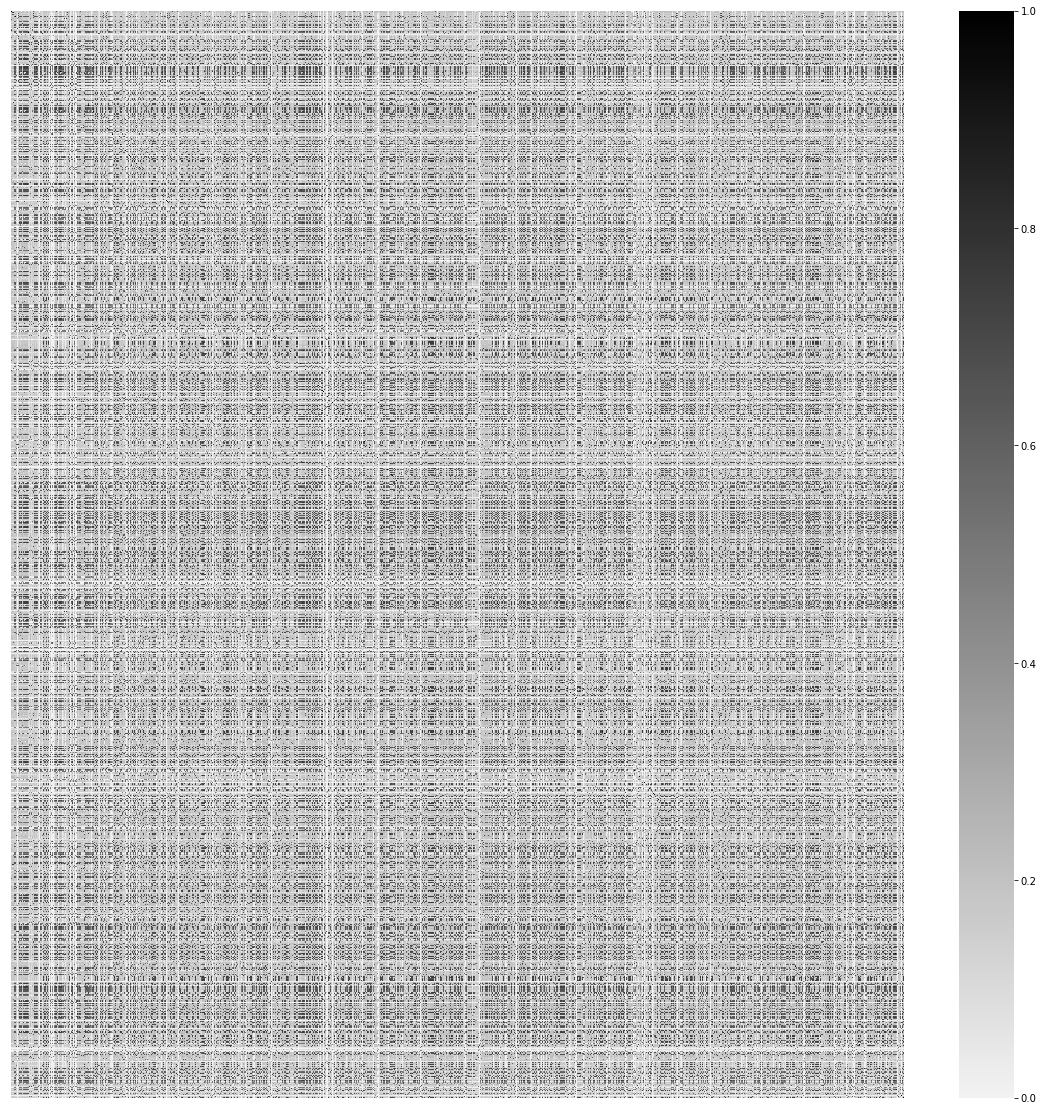
\includegraphics[width=6cm]{event_sim.png}
  \caption*{热力图}
  \label{ff1}
  \end{minipage}
  \begin{minipage}[t]{0.48\textwidth}
  \centering
  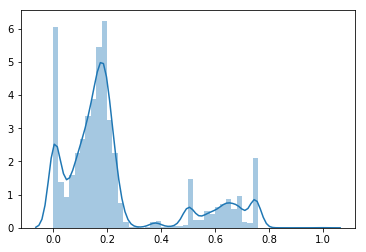
\includegraphics[width=6cm]{event_sim_dist.png}
  \caption*{分布}
  \label{ff2}
  \end{minipage}
  \caption{实验结果}
\end{figure}

可以看出相似矩阵值在0.5附近有较大的差异,并且分布比例也恰好在8:2左右,因此我们把阈值取为0.5。然后我们通过事件成功的定义来对所有事件的成功性进行标注。

\subsubsection{训练分类器}
为了初步的衡量事件的描述对事件参与人数的影响,我们可以将描述作为一个可选的属性,使用一些常用的分类器,例如随机森林,adaboast,对事件成功性进行预测。这里输入是向量化后事件的属性,输出是之前的标注结果。为了避免稀疏高维的文本向量对分类效果的影响,这里对文本的处理方式参考了第二节所用的方法,即事先训练好一个拉索回归器,使用该回归器产生的值来取代原始文本。关于分类器的介绍可以参考附录A。

最终我们使用adaboost,决策树,knn和随机森林作为分类器,使用4折交叉验证来衡量结果,使用网格搜索来确定最佳参数。
本次实验平台为i5-4200m,内存为8G,显卡为gtx-730m。实验结果如图(\ref{f3}):

\begin{figure}
\centering
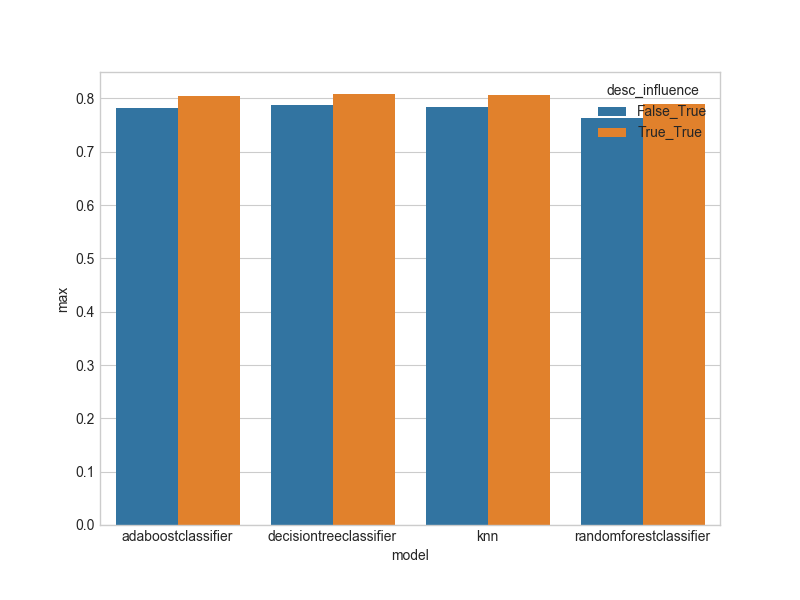
\includegraphics[width=10cm]{exp4_with_1.png}
\caption{}
\label{f3}
\end{figure}

通过实验结果可以看出,加入了事件描述后,分类的精度有了提高。注意到这里排除了相同事件,所以提高的原因不是因为相同事件之间参与人数的相似性。由此可以得出结论:事件描述对预测事件成功起正面作用。

但同时我们也可以看出,事件描述对结果的提高是有限的。这是由于多种原因造成的:一是由于文本处理的方式过于粗糙,二是由于样本太少(交叉验证时每次训练量大概只有3000条),三是由于样本分布不均匀(大概75\%的事件是负样本)。除此以外还有一个很重要的原因:事件描述在某些情况下并不是那么重要。能影响事件参与人数的因素非常多,而在某些情况下,当其他因素起决定性作用的时候,事件描述的好坏就不再是那么重要的了。

想要说明事件描述的影响,光凭分类结果的提升是不够的,引入事件描述对结果最直接的影响是引入了更多的信息,从而提高了分类结果,但有可能并没有提高模型的解释度。为了解决这个问题,我们又设计了如下实验。在介绍接下来的实验前,我们先简单介绍一下线性混合模型。

\subsubsection{线性混合模型}

线性混合模型(\textit{Linear mixed model})是对线性模型的扩展。通过增加固定效应和随机效应,线性混合模型能很好的表示数据中某些非独立的属性对结果的影响。例如性别对于身高来说就是非独立的属性。而对应本文中所使用的数据,就是事件种类,举办地点等属性作为离散变量对于事件参与人数是非独立的。但是事件描述和组内人数则是相对独立的,因此在这里使用线性混合模型来描述这些属性和参与人数的关系是非常自然的一件事情。

\subsubsection{建立混合模型}

为了能更进一步的说明事件描述的加入提高了模型的解释能力,我们使用了混合模型对参与人数与事件的属性之间的关系进行描述。注意到这里我们并不是想根据事件去推算参与人数,而是想给予此判断事件描述在整个模型中起的作用。我们建立的混合模型如下:

\begin{equation}
y_{ijkm}=\beta_0+log|g_i^m|+\gamma_j+\alpha_k+ (\phi_m) +\epsilon_{ijkm}
\end{equation}

其中\(\gamma_j\),\(\alpha_k\)和\(\phi_m\)为事件主题,事件举办人和事件描述的随机效应,固定效应为组内人数。这里没有将事件举办地点纳入考虑范围是因为事件举办地点太多,大多数情况下事件的举办地点都不一样,如果将其考虑进来,会使样本过于稀疏,降低模型的解释性。

Nakagawa和Schielzeth\cite{nakagawa_ageneralandsimplemethodforobtaining_2013}提出了衡量混合模型中的确定系数\(R^2\),在混合模型中,确定系数分为两种,一是\(R_m^2\),衡量固定效应对模型的作用,二是\(R_c^2\),衡量所有效应对模型的作用。计算方法如下:

\begin{equation}
R_m^2=\frac{\sigma_m^2}{\sigma_m^2+\sigma_\gamma^2+\sigma_\alpha^2+(\sigma_\phi^2)+\alpha_\epsilon^2}
\end{equation}
\begin{equation}
R_c^2=\frac{\sigma_m^2+\sigma_\gamma^2+\sigma_\alpha^2+(\sigma_\phi^2)}{\sigma_m^2+\sigma_\gamma^2+\sigma_\alpha^2+(\sigma_\phi^2)+\alpha_\epsilon^2}
\end{equation}

其中\(\sigma\)为方差。我们使用了R语言中的``lme4''计算包\cite{lme4}实现模型,\(R^2\)的计算使用了R语言中的``MuMIn''计算包\cite{MuMIn}。结果如表(\ref{t3})。

\begin{table}[htbp]
	\centering
  \caption{}
  \label{t3}
	\begin{center}
    \begin{tabular*}{\linewidth}{p{0.33\linewidth}p{0.33\linewidth}p{0.33\linewidth}}
  \toprule
                           &  \(R_c^2\) & \(R_m^2\) \\ 
  \midrule
		包含事件描述                       & \textbf{0.653} & 0.135 \\ 
    不包事件含描述                        & 0.494 & 0.135 \\ 
  \bottomrule
    \end{tabular*}
  \end{center}
\end{table}

可以看出包含事件描述后,\(R_c^2\)显著提高,这说明加入了事件描述后,模型的解释性得到了增强。另一个值得注意的是组的规模对事件参与人数并没有特别显著的影响。

\subsection{小结}
本文定义了事件相似性,并使用拉索回归对事件描述进行回归,得到了可解释的结果。然后使用一系列分类器证明了事件描述可以帮助提高预测事件参与度的准确率,最后使用了混合模型证明了该提升并不只是增加了多余的信息,而是提高了模型的解释能力,由此得出事件描述是影响事件是否成功的非常重要的一环的结论。因此,正如前文所描述的,写好一个事件描述,对于sh

然而,值得注意的是,这里我们使用的方法仍然是十分简略的,拉索回归虽然可以得到可解释性的结果,但其简单的特性也导致了其会损失很多信息,例如文本中的序列信息。而这些信息对于提升事件参与度的判定是十分重要的。所以接下来,我们会去尝试更复杂的模型,看看能否在不考虑其他因素的情况下,仅凭借事件描述这一属性,就推测出事件的参与度来。这在现实中也是有意义的:事件组织者可以借助这种工具来预估事件参与人数,以更好的准备举办事件的前期工作。这部分工作将在第二章得到足够多的阐述。

另一个值得注意的地方是如何产生更好的事件描述的工作。近年来在机器翻译,新闻自动撰写等方面的文本生成工作获得了长足的发展,借助序列到序列和对抗网络,我们可以生成可用的,质量足够高的文本。这也启示了我们:一方面,帮助事件组织者判断他们的事件描述是否足够好是有意义的工作,但是如果能自动生成一些有意义的事件描述,也是件有趣的事情。我们将在第三章介绍这部分工作。

总的来说,通过上述实验和方法,我们验证了事件描述对事件参与度是有显著影响的。

% \end{document}